 \chapter{Recerca prèvia}
\label{c:intro}
\section{La Història de la Intel·ligència Artificial: Des dels Orígens fins Avui}
\subsection{El Naixement d'una Idea Revo lucionaria (1956)}
Tot va començar amb una pregunta provocadora d’Alan Turing, el geni matemàtic que va desxifrar Enigma, una màquina emprada pels nazis per codificar els seus missatges durant la Segona Guerra Mundial (1939-1945): "Podran les màquines pensar alguna vegada?". Aquesta qüestió va obrir les portes a un nou camp d’estudi. En 1956 John McCarthy, Marvin Minsky i d'altres especialistes van nominar oficialmenta el terme ``Inteligencia artificial'' durant la famosa conferencia de Darmouth, marcant el inici d'una nova era tecnologica.
\subsection{El Joc que ho va canviar tot: The Imitation Game/El test de Turing}
El nucli de la IA es basa en un experiment molt senzill però profund:El joc d'imitació(The imitation game), proposat per Alan Turing. Davant de la pregunta "Podran les màquines pensar alguna vegada?", Turing va dissenyar un joc que funcionava com a test per les màquines anomenat ``The Imitation Game''. Aquest test consistia en que un avaluador havia de començar una conversa en forma de textos escrits amb una persona i una máquina durant 5 minuts, aquest avaluador no sabia qui era qui i el seu objectiu era esbrinar qui era l'humà. Si la màquina aconseguia enganyar a l'avaluador pasaba el test i es reconeixia que la màquina havia aconseguit un nivell de comportament lingüístic equivalent a la d'un humà, i donava resposta a la pregunta d'Alan Turing. Al cap dels anys, el joc ha estat evolucionant i moderat per els prodigis de la humanitat fins que avui en dia es conegut com el test de Turing. Tot això va ser clau en  donar lloc al naixement de la IA i per l'avanç de la tecnologia.
\subsection{ELs grans fites de la IA}
\subsubsection{1997: La maquina que va vencer un campio}
 La supercomputadora Deep Blue desnvolupada per IBM va derrotar el campió mundial d’escacs, Garry Kasparov, demostrant que la IA podia superar els humans en jocs d’estratègia complexos.
\subsubsection{2022: L'explosió de la IA}
Milions d’usuaris van descobrir models com ChatGPT que podien escriure, traduir i programar amb un llenguatge gairebé humà, obrint nous horitzons en la interacció home-màquina.
\subsubsection{2025: La IA en tots els ambits}
    2025: La IA en Tots els Àmbits
    Avui, la IA està present en dibuix, contingut audiovisual, cotxes autònoms, medicina i molt més, amb models cada vegada més especialitzats i avançats.



(Fonts: \cite{McCarthy_Minsky_Rochester_Shannon_2006}, \cite{deep-blue},
\href{https://openai.com/index/chatgpt/}{ChatGPT (2022)},
\cite{10.1093/mind/LIX.236.433}
)

\section{Que és la Ia?}
Hem estat parlant molt durant aquest treball sobre la IA, i ara que em après quina és la seva història, hem de saber que és. Doncs bé, podem definir la IA com sistemes de software i de hardware disenyats per humans que actúen en un la dimensió física o digital, es a dir, raonar sobre el coneixemen, processant la informació derivada de dades i prendre les millors decisions per assolir l'objectiu donat. O dit d'un altre manera, és un camp de la informàtica que consisteix en un conjunt de capacitats interectuals i cognitives expresades per un sistema informàtic creat pels humans que té com a proposit imitar la intel·ligència humana, com escriure poemes, reconeixer imatges, fer prediccions basades en dades i més funcions. Un exemple de IA i que tot el món coneix i utilitza és el ChatGPT, un chatbot impulsada per un model d'intel·ligència artificial generativa de la empresa OpenAI. Utilitza técniques de processament de llenguatge natural per comprendre preguntes fetes per l'usuari i generar respostes coherents en converses, simulant una interacció similar a la d'un humà. Aquesta IA ha avançat molt desde el seu llençament, ara pot generar o editar imatges, procesar audios, llegir arxius, comrendre imatges i molt més.

\section{Com funciona la IA?}
Una vegada que ja sabem que és una IA, ens toca entendre com funciona. Les intel·ligències arficials utilitzen algoritmes i models matemàtics per processar grans quantitats de dades i prendre accions basades en patrons i regles establertes a travès de l'aprenentatge automàtic o l'aprenentatge profund. Per tant per funcionar necessitara:  \nameref{subsec:Dades}  \ \nameref{subsec:Algorismes}  \ \nameref{subsec:Potència de còmput} \ \nameref{subsec:Software i Frameworks} \ \nameref{subsec:Optimització i Ajustos}  \ \nameref{subsec:Aplicació pràctica} \ \nameref{subsec:Ètica i Regulació}

\subsection{Dades}\label{subsec:Dades}
Les dades son fonamentals per la IA ja que es la base de l'aprennetatge del model, per poder raonar, prendre decisions, i millorar la presició. Aquí esdevenen uns exemples que pot haver:

\subsubsection{Basé d'aprenentage}
\begin{itemize}
 \item Les algoritmes de la IA necessiten a base de dades i una gran diversitat de dades per poder identificar patrons i construir prediccion.
\end{itemize}
\subsubsection{Qualitat vs Quantitat}
\begin{itemize}
\item Una gran quantitat de dades ajudaran a la IA a obtendendre major precisió, però la qualitat es encara més important per la complexibilitat de dades que aporta, això evitara que la IA cometes errors per informacio incompleta.\textbf{ Per exemple:} {\color{blue}En l'ambit medic si vols que la IA fagi una predicció i tan sol li dones una quantitat important de persones sanes i no d'altres exemplars, la IA simplement descartara d'altres possibilitats que podrian haver i només agafar la sana.}
\end{itemize}
\subsubsection{Exemples Reals}
\begin{itemize}
 \item Les sistemes dels cotxes o assistents virtuals necessiten dades en temps reals per adaptar-se de l'entorn, també plataformes com Netflix o Spotify necessiten dades personalitzades per poder generar recomanacions amb presició.
\end{itemize}
\subsubsection{Legisme i Etica}
\begin{itemize}
 \item A la IA s'ha d'aplicar dades com protecció de dades per favorir l'etica i moral, i se li ha d'entrenar amb fonts legitima, valides per tal d'evitar erros legals o tecnics
\end{itemize}


\subsection{Algorismes}\label{subsec:Algorismes}

\subsubsection{L'aprenentage automàtic(Machine learning)}
\begin{itemize}
 \item L'aprenentatge automàtic és una branca crucial de la intel·ligencia artificial, consisteix en cobrar vida a la maquina, donar-li el poder d'aprenentatge dels humans, realitzar tasques de manera autonoma i finalment les infinites possibilitats de evolucionar a traves de l'experiencia i molt més dades. Segons la \href{https://ischoolonline.berkeley.edu/blog/what-is-machine-learning/}{UC Berkeley} el procéss automatic es pot dividir-se en tres parts:
  \begin{enumerate}
  {\color{gray}
   \item \textbf{Mecanisme de predicció}
    \subitem\hspace*{-1\leftmargin} Un conjunt de regles o operacions matemàtiques que analitza les dades d'entrada i intenta identificar els patrons que busca el model.
   \item \textbf{Funció de pèrdua (o error)}
   \subitem\hspace*{-1\leftmargin} Un sistema per avaluar l'encert de les prediccions, comparant-les amb resultats reals (quan es disposa d'ells). Si la predicció és incorrecta, aquesta funció quantifica la magnitud de l'error.
   \item \textbf{Algorisme d'optimització}
   \subitem\hspace*{-1\leftmargin} El procés que ajusta automàticament el model per minimitzar l'error, modificant els paràmetres interns per millorar les prediccions futures.} \ \footnote{Llengua original: Anglessa; Traduit per el chat bot Deepseek}
  \end{enumerate}
  Segons \href{https://blogs.nvidia.com/blog/supervised-unsupervised-learning/}{Nvidia} hi han molts tipus d'apranentage automatics:
  \begin{description}
   \item \nameref{subsubsec:Aprenentatge supervisat}
   \item \nameref{subsubsec:Aprenentatge semi-supervisat}
   \item \nameref{subsubsec:Aprenentatge no supervisat}
   \item \nameref{subsubsec:Aprenentatge reforç}
  \end{description}
\subsubsection{Aprenentatge supervisat}\label{subsubsec:Aprenentatge supervisat}
L'aprenentatge supervisat és un tipus d'aprenentatge automàtic que treballa amb dades etiquetades, és a dir, dades que ja inclouen la solució o resultat desitjat. En aquest mètode, la intel·ligència artificial aprén a associar les dades d'entrada amb les seves etiquetes corresponents, mitjançant l'anàlisi d'exemples prèviament resolts. Això li permet desenvolupar la capacitat de resoldre problemes nous aplicant la lògica i els patrons identificats a partir de dades reals.\\
Avantatges i desavanantatge:
Aquest mètode destaca per la seva alta precisió en problemes ben definits, ja que al treballar amb dades prèviament etiquetades pot assolir bons resultats en tasques de classificació i regressió. Una altra avantatge important és la facilitat per avaluar el rendiment dels models. A més, es tracta d'una àmplia àrea d'estudi amb una gran varietat d'algoritmes ben desenvolupats i optimitzats, com ara els arbres de decisió, els random forests, les màquines de vectors de suport (SVM) o les xarxes neuronals. Finalment, un cop entrenat adequadament, el model pot generalitzar el seu aprenentatge i fer prediccions útils sobre dades noves.

No obstant això, aquest enfocament també presenta alguns inconvenients significatius. El principal desavantatge és la seva forta dependència de conjunts de dades etiquetades, que sovint són costosos d'obtenir i preparar com las de medicines. Un altre problema freqüent és el sobreajustament (overfitting), que ocorre quan el model memoritza les dades d'entrenament en lloc d'aprendre patrons generals, la qual cosa provoca una perdua de raonament logica. Finalment, aquest mètode pot tenir dificultats per manejar certs tipus de dades no estructurades o problemes complexos, que podrien requerir quantitats molt grans de dades etiquetades per assolir un bon rendiment.


\subsubsection{Aprenentatge semi-supervisat}\label{subsubsec:Aprenentatge semi-supervisat}

L'aprenentatge semi-supervisat representa un punt intermig entre l'aprenentatge supervisat i el no supervisat, aprofitant tant dades etiquetades com no etiquetades per millorar l'eficiència dels models d'aprenentatge automàtic. Això funciona quan l'obtencio de les dades etiquetades son molt costoses i l'extraccio de les característiques son molt complexes.
\subsubsection{Aprenentatge no supervisat}\label{subsubsec:Aprenentatge no supervisat}

L'aprenentatge no supervisat és una branca de l'aprenentatge automàtic que s'utilitza quan no es disposa de dades etiquetades. A diferència de l'aprenentatge supervisat, on el model rep exemples amb les seves solucions correctes, en aquest cas l'algorisme ha de descobrir per si mateix l'estructura i els patrons, fent una diagnosticació agrupant les característiques similars que poden haber entre les dades.

Depenen dels tipus de  problemes, les dades s'organitzen de diferents maneres.
\begin{itemize}
 \item \textbf{Clustering:} Tècnica que agrupa les dades en funció de les seves similituds.
 \item \textbf{Anomaly detection:} Cerca patrons que no encaixen amb el comportament normal.
 \item \textbf{Association:} Cerca relacions i correlacions entre variables en grans conjunts de dades.
 \item \textbf{Autoencoders:} Els autoencoders són un tipus de xarxa neuronal artificial que aprèn a comprimir i reconstruir dades.
\end{itemize}


\subsubsection{Aprenentatge reforç}\label{subsubsec:Aprenentatge reforç}
L'aprenentatge per reforç és una branca de l'aprenentatge automàtic inspirada en la manera com els éssers vius aprenen mitjançant la interacció amb el seu entorn. Com per exemple quan començem a jugar un videojoc, en els jocs rebem senyals de reforços, de si completem un nivell ens ortoga un trofeu, de si matem certs enemics guanyem bonificacions. Amb aquest sistema de penalitzacio i recompenses guia al jugador a millorar les seves tecniques de videojocs , i això  el podem aplicar perfectament en la IA.
Totes les aprenantatges de reforç segueixen pragmaticament aquest esquema per l'aprenentage:
\begin{enumerate}
 \item Acció
 \item Observació
 \item Recompensa
 \item Ajust d'estrategia
\end{enumerate}




\end{itemize}

\subsubsection{L'aprenentatge profund}
\begin{itemize}
 \item L'aprenentatge profund és una branca de l'aprenentatge automàtc, utilitza xarxes neuronals explicat en l'apartat \ref{sec:3.3} amb múltiples capes per procesar dades complexes i extraure característiques rellevants, això permet a la IA realitzar tasques com el reconeixement d'imatges.
\end{itemize}
\subsection{Potència de còmput}\label{subsec:Potència de còmput}
\begin{itemize}
 \item Hardware potent: GPUs (unitats de processament gràfic) o TPUs (Tensor Processing Units) per accelerar els càlculs.
 \item Infraestructura en núvol: Moltes IA es executen en servidors remots amb gran capacitat de processament.
\end{itemize}

\subsection{Software i Frameworks}\label{subsec:Software i Frameworks}
\begin{itemize}
 \item Llibreries especialitzades: TensorFlow, PyTorch, scikit-learn, etc.
 \item Llenguatges de programació: Python (el més comú), R, Julia, etc.
\end{itemize}

\subsection{Optimització i Ajustos}\label{subsec:Optimització i Ajustos}
\begin{itemize}
 \item Ajust de hiperparàmetres: Per millorar la precisió del model.
 \item Validació i proves: Assegurar que la IA funcioni correctament en diferents escenaris.
\end{itemize}
\subsection{Aplicació pràctica}\label{subsec:Aplicació pràctica}
\begin{itemize}
 \item Integració amb sistemes existents: Per exemple, en robòtica, salut, finances, etc.
 \item Interfícies d'usuari: Com chatbots, aplicacions mòbils o sistemes de recomanació.
\end{itemize}
\subsection{Ètica i Regulació}\label{subsec:Ètica i Regulació}
\begin{itemize}
 \item Protecció de dades: Complir amb lleis com el GDPR.
 \item Biaixos i justícia: Assegurar que els models no discriminin.
\end{itemize}

Fonts:\href{https://blogs.uoc.edu/digitapia/the-european-unions-artificial-intelligence-act-explained/}{Bloc IA} \href{https://formaciooberta.eapc.gencat.cat/contingutsdelscursos/tdp/080_int_artificial/inici.html}{EAPC Wiki}
\href{https://www.ibm.com/think/topics/machine-learning}{IBM ML}

\section{Que és una xarxa neuronal artificial/biologica?}\label{sec:3.3}
Una xarxa neuronal artificial és un model computacional inspirat en el funcionament del cervell humà, utilitzat en el camp de la intel·ligència artificial (IA) i l'aprenentatge automàtic (machine learning). Està dissenyada per reconèixer patrons, prendre decisions i aprendre a partir de dades, sense ser programada explícitament per a cada tasca específica.
Si tenim una artificial també tindrem una biològica. Una xarxa neuronal biològica es refereix al sistema interconnectat de neurones (cèl·lules nervioses) en el cervell i el sistema nerviós dels éssers vius. Aquestes xarxes són la base de la cognició, l'aprenentatge i les funcions biològiques en humans i animals.
Aquí hi és una taula de comparació entre una biologica i artificial:

\begin{table}[h!]
\begin{tabular}{|l|l|l|}
\hline
\textbf{Aspecte} & \textbf{Xarxa neuronal biològica} & \textbf{Xarxa neuronal artificial} \\ \hline
\textbf{Base} & Cèl·lules vives (neurones). & Algoritmes matemàtics. \\ \hline
\textbf{Energia} & Baix consum (\textasciitilde20 watts). & Alt consum (GPUs/TPUs). \\ \hline
\textbf{Aprenentatge} & Plasticitat sinàptica. & Backpropagation + dades. \\ \hline
\textbf{Velocitat} & Lent (mil·lisegons). & Ràpid (nanosegons). \\ \hline
\end{tabular}
\caption{Comparativa entre xarxes neuronals biològiques i artificials}
\end{table}
Fons: \href{https://www.ibm.com/docs/es/spss-modeler/saas?topic=networks-basics-neural}{https://www.ibm.com/docs/es/spss-modeler/saas?topic=networks-basics-neural}
\section{Estructura d'una xarxa neuronal}
Una xarxa neurnal combina diverses capes de procesament i utilitza elements simples que operen en paral·lel, simulen i estan inspirades en els sistemes nerviosos biològics com hem explican en l'apartat \ref{sec:3.3}. Consta d'una capa d'entrada, seguit d'una o varies capes ocultes i finalment una capa de sortida. Les capes estan interconectades mitjançant nodes o neurones; cada capa utilitza la sortida de la capa anterior com a entrada.

\begin{itemize}
 \item \textbf{Capa d'entrada:}La capa d'entrada és la primera capa que reb directament la informació d'entrada que es prcessarà. Aquesta capa no realitzarà càlculs complexos, simplement transmet les dades a les capes seguents per fer el processament.
 \item \textbf{Capes ocultes:}Les capes ocultes són les capes que estan entre la capa d'entrada i la de sortida, aquestes capes contenen unitats no observables. La seva funció principal és processar les dades de la capa d'entrada per extraure característiques i patrons complexos. Aquestes capes són els que realitzan els càlculs i permet que la xarxa aprengui relacions no lineals i representacions abstracts de les dades, això és molt important per fer tasques complexes com el reconeixement de patrons.
 \item \textbf{Capa de sortida:}La capa de sortida és l'última capa que forma una xarxa neuronal i és l'encarregada de produïr la predicció final del model. Aquesta capa utilitza la informació que ha processat la o les capes ocultes i la transforma a travès d'una funció activa per generar una sortida, que pot ser una predicció numèrica, una clasificació o qualsevol altre resultat.
 \end{itemize}


\begin{figure}[h!]
    \centering
    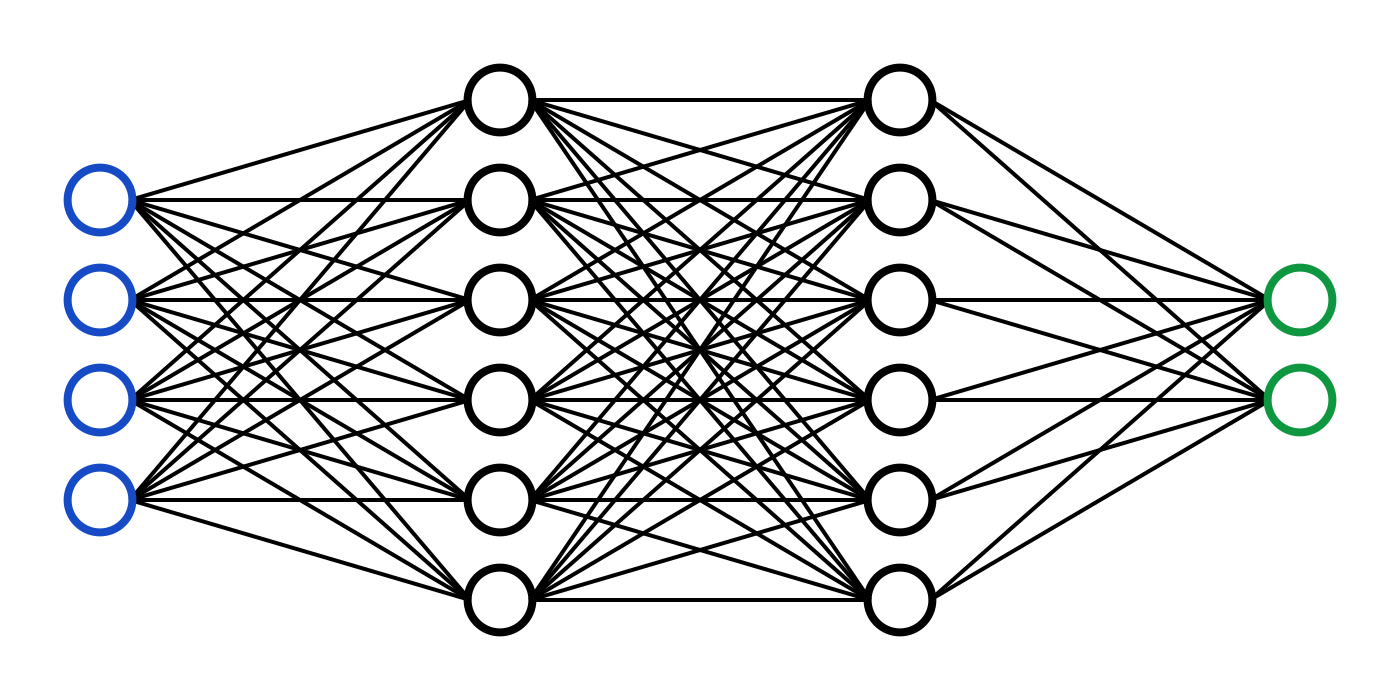
\includegraphics[width=0.5\textwidth]{./figures/xarxa.png}
    \caption{Estructura d'una xarxa neuronal}
\end{figure}

Fons: \href{https://msmk.university/hidden-layer/}{https://msmk.university/hidden-layer/}

\href{https://www.linkedin.com/advice/0/what-some-examples-linear-nonlinear-models-real-world?lang=es&lang=es&originalSubdomain=es}{Article Linkedin}

\section{Funció d'activació}\label{sec:3.5.3}
Les funcions d'activació són un component integral de les xarxes neuronals que els permeten aprendre patrons complexos en les dades. Transformen el senyal d'entrada d'una neurona en un senyal de sortida que passa a la capa següent. Sense funcions d'activació, les xarxes neuronals es limitarien a modelar únicament relacions lineals entre entrades i sortides, és a dir, introdueixen la no linealitat i produeixen la sortida de la neurona.

\subsection{Funció sigmoide}
Una funció d'activació molt coneguda és la funció sigmoide. La seva fórmula és:
\[ \sigma(x) = \frac{1}{1 + e^{-x}} \]

Aquesta funció matemàtica transforma qualsevol valor d'entrada real en un valor que està 0 i 1. La seva forma característica és una curva en forma de ``S''. Si el valor de $x$ que introduïm a la funció és molt gran o fins infinit $(\infty)$, llavors\ $\sigma$ serà 1; en canvi si és molt petit o menys infinit $(-\infty)$,\ $\sigma$ serà 0, i si x = 0,  $\sigma$  serà 0,5.

\begin{figure}[h!]
    \centering
    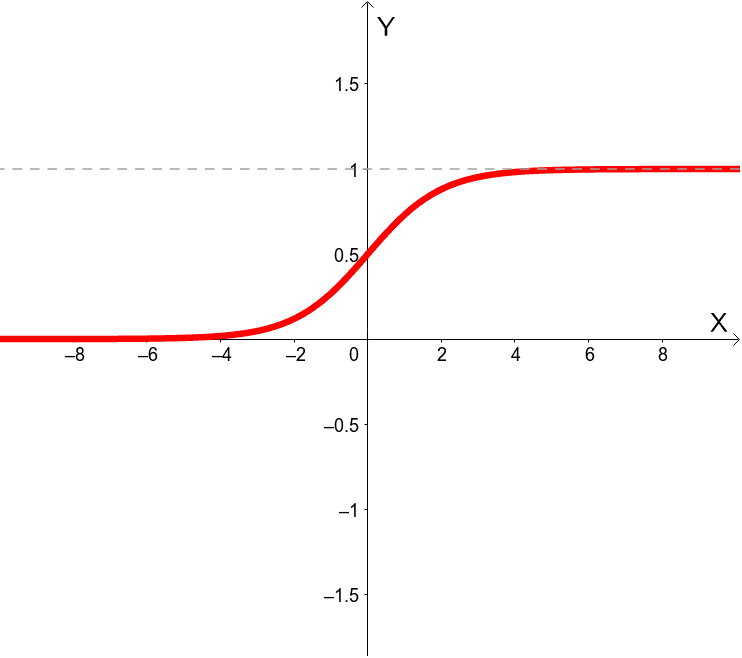
\includegraphics[width=0.5\textwidth]{./figures/grafica_sigmoide.png}
    \caption{Gràfica de la funció sigmoide}
\end{figure}

\textbf{Avantatges:}
La avantatge principal de la funció sigmoide és la seva suavitat i la facilitat de derivació. La funció és diferenciable en tots els punts, això vol dir que permet als algoritmes d'optimització treballar amb la funció de manera eficient. A més, la funció és monòtona creixent, ho que significa que una entrada major sempre produirà una sortida major, fent que sigui útil per modelar relacions de causa i efecte.

\textbf{Desavantatges:}
Tanmateix, la funció sigmoide també té algunes desavantatges. Un dels seus problemes és que la funció es satura quan els valors d'entrades són grans, ho que significa que la derivada de la funció s'apropa a 0 i l'aprenentatge es relentitza. Un altre problema és que aquesta funció no és simètrica, causant a les entrades negatives i positives es processin de mandera diferent, això pot afectaral rendiment de la xarxa.
\subsection{Funció ReLU(Funció Uniat Rectificada Uniforme)}
La funció Unitat Rectificada Uniforme té la fòrmula seguent:
\[ f(x) = \max(0, x) \]

Aquesta funció té l'algoritme seguent: Si el valor d'entrada es menor que 0, mostra 0, si el valor d'entrada es major o igual que 0, mostrarà el valor d'entrada. Això vol dir que la funció és lineal si la entrada és més gran que 0 perquè la pendent és 1. Encara que la funció ReLU és lineal per a la mitat del seu espai d'entrada, tècnicament és una funció no lineal perquè té un punt no diferenciable en x = 0, on canvia bruscament respecte a x. Aquesta no linealitat permet a les xarxes neuronals apendre patrons complexos.

\begin{figure}[h!]
    \centering
    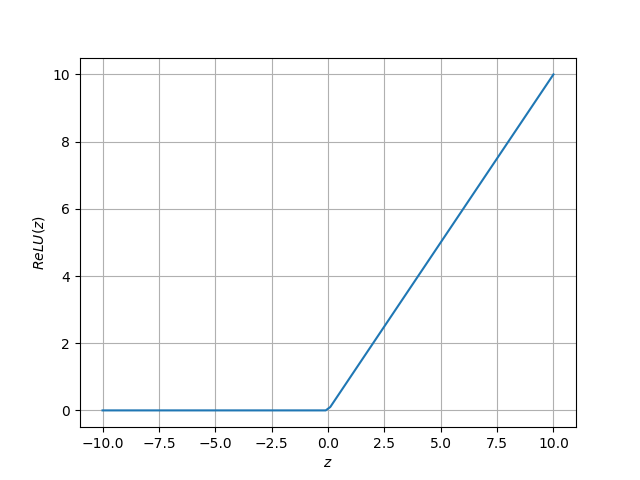
\includegraphics[width=0.5\textwidth]{./figures/ReLU.png}
    \caption{Gràfica de la funció ReLU}
\end{figure}

Tot i això, aquesta funció té una desavanantatge; si utilitzen la funció ReLU com a funció d'activació pasarà una cosa, i es que tots els valors negatius són 0, per tant en el procès de retroprogramació, explicat a l'apartat \ref{sec:3.6.1}, no es produeix els valors d'ajust en les neurones negatives. Per solucionar aquest problema s'ha inventat una nova funció que es diu Leaky ReLU. Funciona igual com l funció ReLU, però té un valor determinat per les neurones negatives.

\begin{figure}[h!]
    \centering
    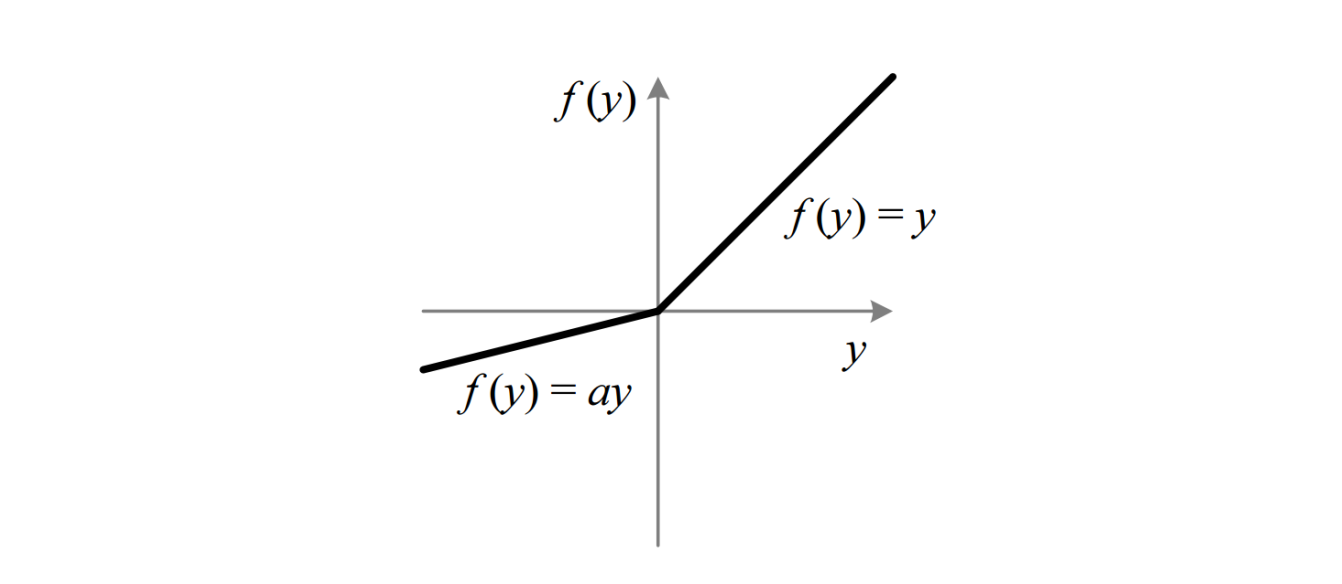
\includegraphics[width=0.5\textwidth]{./figures/leaky_ReLU.png}
    \caption{Gràfica de la funció Leaky ReLU}
\end{figure}

\subsection{Funció Softmax}
La funció Softmax, és una de les funcions que més s'utilitzen en xarxes neuronals i és especialment útil en el context dels problemes de clasificació multiclase. Aquesta funció opera sobre un vector que representa les previsions de cada clase, calculades per les capes anterior.

\begin{figure}[h!]
    \centering
    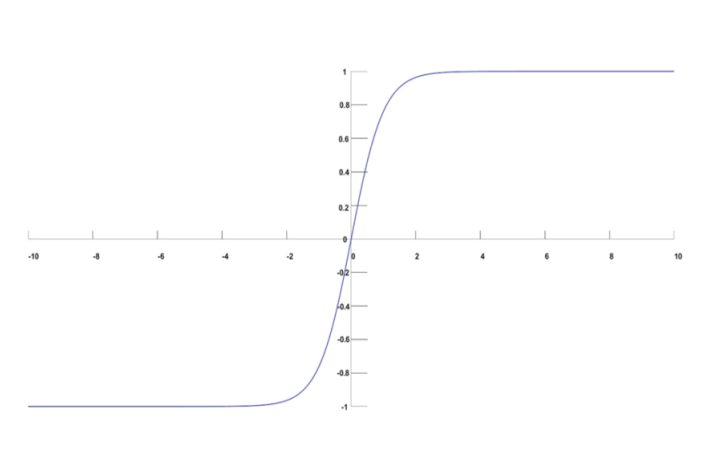
\includegraphics[width=0.5\textwidth]{./figures/Softmax.png}
    \caption{Gràfica de la funció Softmax}
\end{figure}

Per a un vector d'entrada x amb elements x1, x2,..., xC, la funció Softmax es defineix com:
\[f(x_i) = \frac{e^{x_i}}{\sum_{j=1}^{n} e^{x_j}}\]

El resultat de la funció Softmax és una distribució de probabilitat de la quàl la suma és 1. Cada element del resultat representa la probailitat de que l'entrada pertanyi a una clase determinada. L'ús d'aquesta funció garantitza de que tots els valors de la sortida siguin positius. Això és molt important perquè les porbabilitats no poden ser negatives.

\begin{figure}[H]
    \centering
    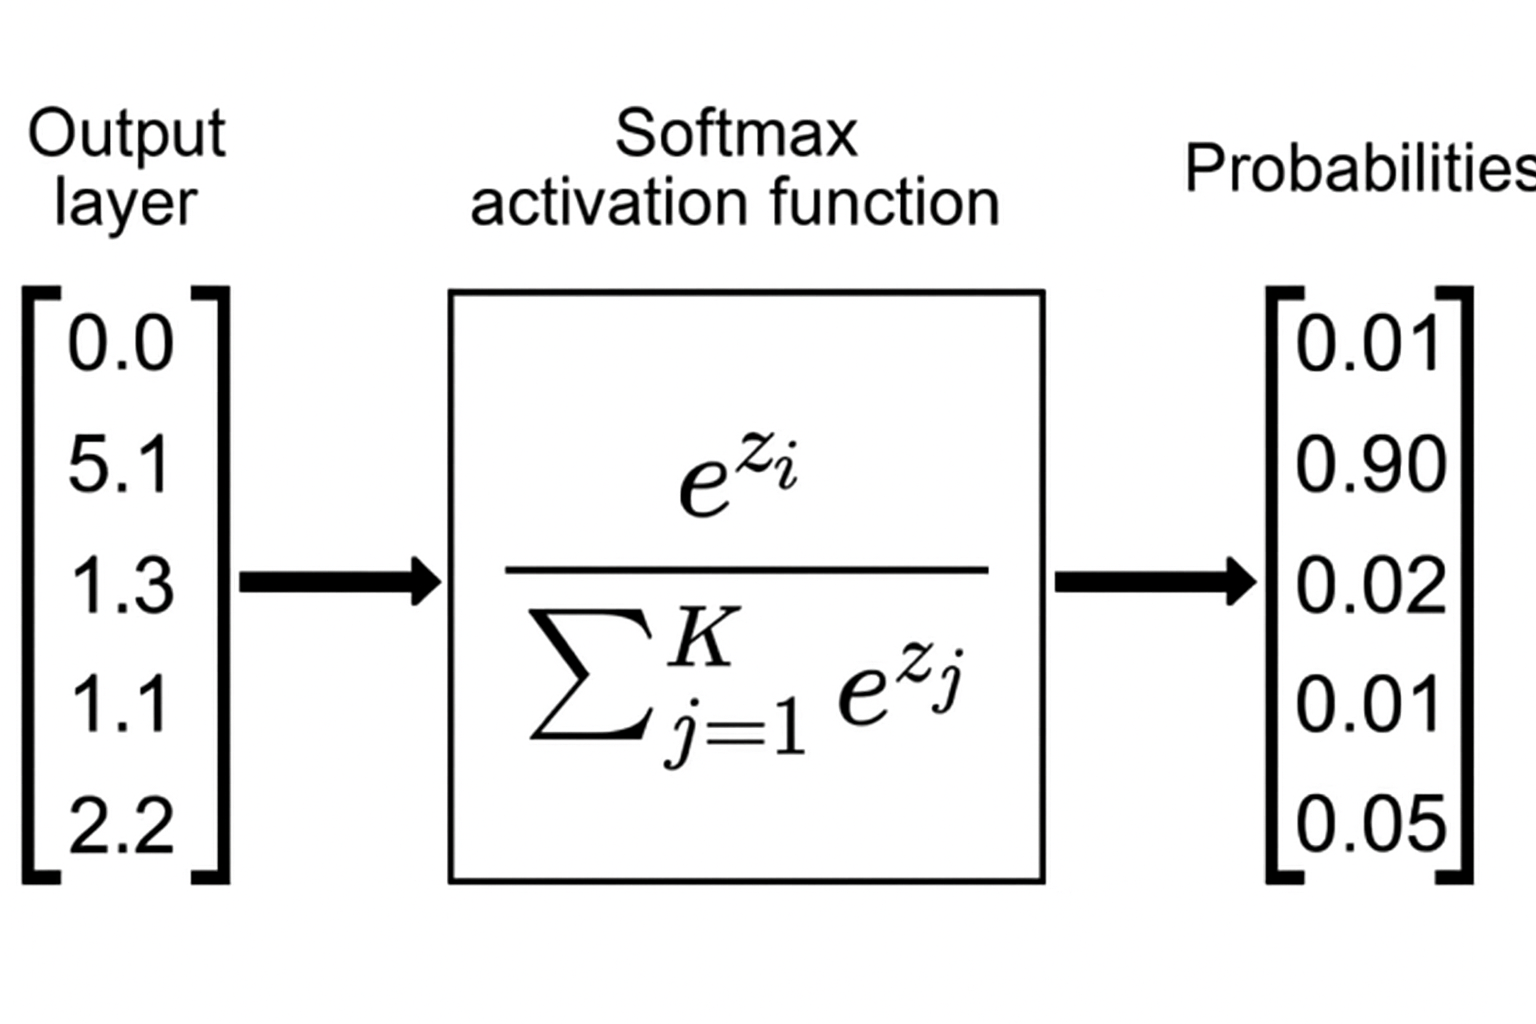
\includegraphics[width=0.5\textwidth]{./figures/representacio_Softmax.png}
    \caption{Representació de la funció Softmax}
\end{figure}

Fons: \href{https://msmk.university/hidden-layer/}{https://msmk.university/hidden-layer/}


\href{https://jacar.es/la-funcion-sigmoide-una-herramienta-clave-en-redes-neuronales/}{https://jacar.es/la-funcion-sigmoide-una-herramienta-clave-en-redes-neuronales/}

\section{Com funciona una xarxa neuronal?}
Ara que sabem quina estructura forma una xarxa neuronal artificial, toca entendre com funciona. Les neurones o nodes son els pilars més importants d'una xarxa neuronal. Cada neurona utilitza la entrada, la processa fent una suma ponderada entre els pesos i les entrades, després una funció d'activació, i pasa la sortida a altres neurones.

Les conexions(pesos i biaix) son la força de conexió entre dos neurones representades per un pes. Els pesos son valors que determinen cuánta influència té la producció d'una neurona sobre un altre. Els biaixos són paràmetres adicionals que ajude a ajustar la sortida de les neurones.

Per entendre-ho millor, donarem un exemple: Imagina que vols utilitzar una XNA profund que aprengui a reconeixer dígits escrits a mà des de l'ú fins al nou. Per la capa d'entrada, cada neurona d'aquesta capa representaria un píxel de la imatge. Seguit d'això, les capes ocultes serien les encarregades de processar aquesta informació de píxels, identificant característiques com curves, línies, o bucles que conforman els diferents dígits. Finalment, cada neurona de la capa de sortida representaria un dels deu dígits. La neurona amb la activació més alta indicarà la predicció de la xarxa.

Les xarxes neuronals operen a travès d'un procès de dos pasos: La propagació directa i la retropropagació.

\subsection{Propagació directa}
Durant la propagació directa, les dades ingresen en la xarxa a travès de la capa d'entrada i flueixen secuencialment a travès de les capes ocultes fins a la capa de sortida. En cada neurona, els valors d'entrada del model es multiplican per els seus pesos corresponents i es sumen. Aquesta suma ponderada es pasa a travès d'una funció d'activació, explicada prèviament a l'apartat \ref{sec:3.5.3}. Aquest procès continua capa per capa, això acaba conduïnt cap a la predicció final en la capa de sortida.
\subsection{Retroprogramació}\label{sec:3.6.1}
Mentre que la programació directa fa prediccions, la retroporgramació és la forma en que la xarxa apren d'errors. Implica comparar la predicció de la xarxa amb el valor objectiu real i calcular unterme d'eror mitjançant una funció de pèrdua.
Aquest error es propaga enrere a travès de la xarxa, començant des de la capa de sortida. Durant aquest procès, la xarxa ajusta els pesos i els baixos de cada connexió en funció de la seva contribució a l'error, amb l'objectiu de minimitzar-lo.
Aquest procès iteratiu de càlcul d'erros i ajustament de pes permet a la xarxa d'aprenentatge profund millorar gradualment les seves prediccions.



